%-*-latex-*-
\sectionthree{Recursive function call}
\begin{python0}
from solutions import *; clear()
\end{python0}

Now let me consider the case of recursive functions.
Recursive functions can take many forms.
I'll focus on three typical cases.

Of course we have to look at Fibonacci:
\begin{Verbatim}[frame=single,fontsize=\footnotesize]
int fib(int n)
{
    if (n == 0 || n == 1)
    {
        return 1;
    }
    else
    {
        return fib(n - 1) + fib(n - 2);
    }
}
\end{Verbatim}
In this case
\[
\texttt{fib(n)} \text{ calls \texttt{fib(n - 1)}, \texttt{fib(n - 2)} \text{ and performs some computation}} 
\]
In general a recurrence that looks like
\[
\texttt{f(n)} \text{ calls \texttt{f(n - 1)} \text{ and performs some computation}} 
\]
or
\[
\texttt{f(n)} \text{ calls } \texttt{f(n - 1)}, \texttt{f(n - 2)} \text{ and performs some computation} 
\]
or
\[
\texttt{f(n)} \text{ calls } \texttt{f(n - 1)}, \texttt{f(n - 2)}, \texttt{f(n - 3)} \text{ and performs some computation} 
\]
or
\[
\texttt{f(n)} \text{ calls } \texttt{f(n - 2)}, ... , \texttt{f(n - 5)} \text{ and performs some computation} 
\]
etc.~are called \defone{linear recursion}.

Here's the function call graph for \verb!fib(4)!:
%-*-latex-*-
\begin{center}
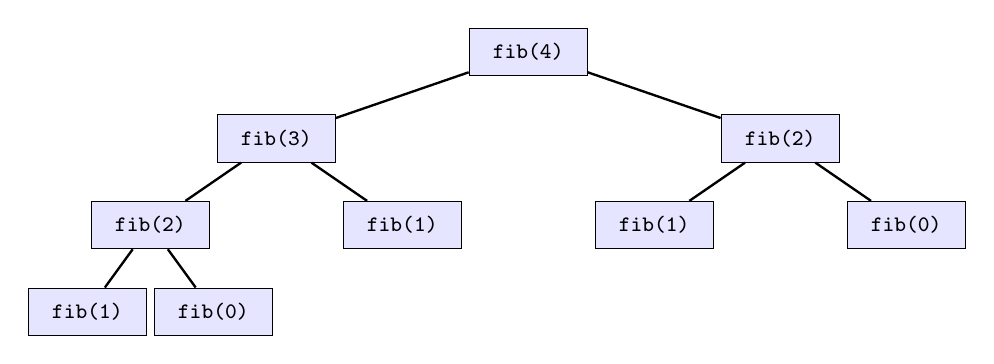
\begin{tikzpicture}

\draw (6.3500000000000005, 0.3)
  node[fill=blue!10,rounded corners=0cm,inner sep=0cm] {

\begin{minipage}[t][0.6cm]{1.5cm}
\mbox{}

\end{minipage}

};
\draw (6.3500000000000005, 0.3)
  node[draw, , , color=black,
       rounded corners=0cm, inner sep=0cm,
       name=A] {

\begin{minipage}[t][0.6cm]{1.5cm}
\mbox{}

\end{minipage}

};\draw (6.3500000000000005, 0.3) node[color=black] {\texttt{{\footnotesize \texttt{fib(4)}}}};
\draw (3.1500000000000004, -0.8)
  node[fill=blue!10,rounded corners=0cm,inner sep=0cm] {

\begin{minipage}[t][0.6cm]{1.5cm}
\mbox{}

\end{minipage}

};
\draw (3.1500000000000004, -0.8)
  node[draw, , , color=black,
       rounded corners=0cm, inner sep=0cm,
       name=B] {

\begin{minipage}[t][0.6cm]{1.5cm}
\mbox{}

\end{minipage}

};\draw (3.1500000000000004, -0.8) node[color=black] {\texttt{{\footnotesize \texttt{fib(3)}}}};
\draw (9.55, -0.8)
  node[fill=blue!10,rounded corners=0cm,inner sep=0cm] {

\begin{minipage}[t][0.6cm]{1.5cm}
\mbox{}

\end{minipage}

};
\draw (9.55, -0.8)
  node[draw, , , color=black,
       rounded corners=0cm, inner sep=0cm,
       name=I] {

\begin{minipage}[t][0.6cm]{1.5cm}
\mbox{}

\end{minipage}

};\draw (9.55, -0.8) node[color=black] {\texttt{{\footnotesize \texttt{fib(2)}}}};
\draw (1.5499999999999998, -1.9000000000000001)
  node[fill=blue!10,rounded corners=0cm,inner sep=0cm] {

\begin{minipage}[t][0.6cm]{1.5cm}
\mbox{}

\end{minipage}

};
\draw (1.5499999999999998, -1.9000000000000001)
  node[draw, , , color=black,
       rounded corners=0cm, inner sep=0cm,
       name=C] {

\begin{minipage}[t][0.6cm]{1.5cm}
\mbox{}

\end{minipage}

};\draw (1.5499999999999998, -1.9000000000000001) node[color=black] {\texttt{{\footnotesize \texttt{fib(2)}}}};
\draw (4.75, -1.9000000000000001)
  node[fill=blue!10,rounded corners=0cm,inner sep=0cm] {

\begin{minipage}[t][0.6cm]{1.5cm}
\mbox{}

\end{minipage}

};
\draw (4.75, -1.9000000000000001)
  node[draw, , , color=black,
       rounded corners=0cm, inner sep=0cm,
       name=F] {

\begin{minipage}[t][0.6cm]{1.5cm}
\mbox{}

\end{minipage}

};\draw (4.75, -1.9000000000000001) node[color=black] {\texttt{{\footnotesize \texttt{fib(1)}}}};
\draw (7.949999999999999, -1.9000000000000001)
  node[fill=blue!10,rounded corners=0cm,inner sep=0cm] {

\begin{minipage}[t][0.6cm]{1.5cm}
\mbox{}

\end{minipage}

};
\draw (7.949999999999999, -1.9000000000000001)
  node[draw, , , color=black,
       rounded corners=0cm, inner sep=0cm,
       name=G] {

\begin{minipage}[t][0.6cm]{1.5cm}
\mbox{}

\end{minipage}

};\draw (7.949999999999999, -1.9000000000000001) node[color=black] {\texttt{{\footnotesize \texttt{fib(1)}}}};
\draw (11.15, -1.9000000000000001)
  node[fill=blue!10,rounded corners=0cm,inner sep=0cm] {

\begin{minipage}[t][0.6cm]{1.5cm}
\mbox{}

\end{minipage}

};
\draw (11.15, -1.9000000000000001)
  node[draw, , , color=black,
       rounded corners=0cm, inner sep=0cm,
       name=H] {

\begin{minipage}[t][0.6cm]{1.5cm}
\mbox{}

\end{minipage}

};\draw (11.15, -1.9000000000000001) node[color=black] {\texttt{{\footnotesize \texttt{fib(0)}}}};
\draw (0.75, -3.0)
  node[fill=blue!10,rounded corners=0cm,inner sep=0cm] {

\begin{minipage}[t][0.6cm]{1.5cm}
\mbox{}

\end{minipage}

};
\draw (0.75, -3.0)
  node[draw, , , color=black,
       rounded corners=0cm, inner sep=0cm,
       name=D] {

\begin{minipage}[t][0.6cm]{1.5cm}
\mbox{}

\end{minipage}

};\draw (0.75, -3.0) node[color=black] {\texttt{{\footnotesize \texttt{fib(1)}}}};
\draw (2.35, -3.0)
  node[fill=blue!10,rounded corners=0cm,inner sep=0cm] {

\begin{minipage}[t][0.6cm]{1.5cm}
\mbox{}

\end{minipage}

};
\draw (2.35, -3.0)
  node[draw, , , color=black,
       rounded corners=0cm, inner sep=0cm,
       name=E] {

\begin{minipage}[t][0.6cm]{1.5cm}
\mbox{}

\end{minipage}

};\draw (2.35, -3.0) node[color=black] {\texttt{{\footnotesize \texttt{fib(0)}}}};\draw[line width=0.03cm,black] (A) to  (B);
\draw[line width=0.03cm,black] (A) to  (I);
\draw[line width=0.03cm,black] (B) to  (C);
\draw[line width=0.03cm,black] (B) to  (F);
\draw[line width=0.03cm,black] (C) to  (D);
\draw[line width=0.03cm,black] (C) to  (E);
\draw[line width=0.03cm,black] (I) to  (G);
\draw[line width=0.03cm,black] (I) to  (H);
\end{tikzpicture}

\end{center}


First let's think about the runtime.
Watchout:
for this section, the \lq\lq runtime of \verb!f(n)!"
refers to the time spent in \verb!f()! and \textit{does not} include
the runtime of the recursive 
\verb!f(n - 1)! and \verb!f(n - 2)!.
For the \textit{next} section,
the \lq\lq runtime of \verb!f(n)!" \textit{will} include
the runtime of the recursive function calls
\verb!f(n - 1)! and \verb!f(n - 2)!.
The second method is more common since there are mathematical techniques
to handle runtime computations for the second method.

Each \verb!f(n)! takes constant time, whether it's the
recursive case or the base cases.
Remember I'm not including the time used in recursive function calls.
Let $A$ be the maximum time of \verb!f(n)!
(i.e., maximum of the time for recursive case and the base cases).
Therefore the total time taken of \verb!f(4)! is
$\text{(the number of function calls)} \times A$.
We're tempted to simplify the counting by adding some rectangles
like this:
%-*-latex-*-
\begin{center}
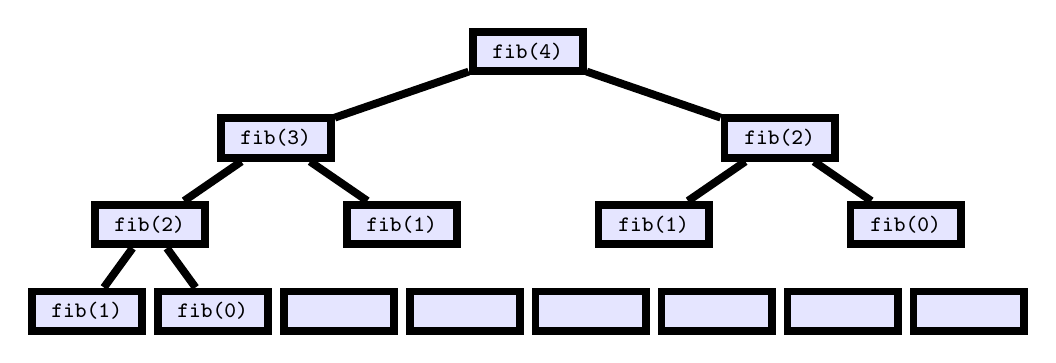
\begin{tikzpicture}

\draw (6.3500000000000005, 0.3)
  node[fill=blue!10,rounded corners=0cm,inner sep=0cm] {

\begin{minipage}[t][0.5cm]{1.4cm}
\mbox{}

\end{minipage}

};
\draw (6.3500000000000005, 0.3)
  node[draw, line width=0.1cm, , color=black,
       rounded corners=0cm, inner sep=0cm,
       name=A] {

\begin{minipage}[t][0.5cm]{1.4cm}
\mbox{}

\end{minipage}

};\draw (6.3500000000000005, 0.3) node[color=black] {\texttt{{\footnotesize \texttt{fib(4)}}}};
\draw (3.1500000000000004, -0.8)
  node[fill=blue!10,rounded corners=0cm,inner sep=0cm] {

\begin{minipage}[t][0.5cm]{1.4cm}
\mbox{}

\end{minipage}

};
\draw (3.1500000000000004, -0.8)
  node[draw, line width=0.1cm, , color=black,
       rounded corners=0cm, inner sep=0cm,
       name=B] {

\begin{minipage}[t][0.5cm]{1.4cm}
\mbox{}

\end{minipage}

};\draw (3.1500000000000004, -0.8) node[color=black] {\texttt{{\footnotesize \texttt{fib(3)}}}};
\draw (9.55, -0.8)
  node[fill=blue!10,rounded corners=0cm,inner sep=0cm] {

\begin{minipage}[t][0.5cm]{1.4cm}
\mbox{}

\end{minipage}

};
\draw (9.55, -0.8)
  node[draw, line width=0.1cm, , color=black,
       rounded corners=0cm, inner sep=0cm,
       name=I] {

\begin{minipage}[t][0.5cm]{1.4cm}
\mbox{}

\end{minipage}

};\draw (9.55, -0.8) node[color=black] {\texttt{{\footnotesize \texttt{fib(2)}}}};
\draw (1.5499999999999998, -1.9000000000000001)
  node[fill=blue!10,rounded corners=0cm,inner sep=0cm] {

\begin{minipage}[t][0.5cm]{1.4cm}
\mbox{}

\end{minipage}

};
\draw (1.5499999999999998, -1.9000000000000001)
  node[draw, line width=0.1cm, , color=black,
       rounded corners=0cm, inner sep=0cm,
       name=C] {

\begin{minipage}[t][0.5cm]{1.4cm}
\mbox{}

\end{minipage}

};\draw (1.5499999999999998, -1.9000000000000001) node[color=black] {\texttt{{\footnotesize \texttt{fib(2)}}}};
\draw (4.75, -1.9000000000000001)
  node[fill=blue!10,rounded corners=0cm,inner sep=0cm] {

\begin{minipage}[t][0.5cm]{1.4cm}
\mbox{}

\end{minipage}

};
\draw (4.75, -1.9000000000000001)
  node[draw, line width=0.1cm, , color=black,
       rounded corners=0cm, inner sep=0cm,
       name=F] {

\begin{minipage}[t][0.5cm]{1.4cm}
\mbox{}

\end{minipage}

};\draw (4.75, -1.9000000000000001) node[color=black] {\texttt{{\footnotesize \texttt{fib(1)}}}};
\draw (7.949999999999999, -1.9000000000000001)
  node[fill=blue!10,rounded corners=0cm,inner sep=0cm] {

\begin{minipage}[t][0.5cm]{1.4cm}
\mbox{}

\end{minipage}

};
\draw (7.949999999999999, -1.9000000000000001)
  node[draw, line width=0.1cm, , color=black,
       rounded corners=0cm, inner sep=0cm,
       name=G] {

\begin{minipage}[t][0.5cm]{1.4cm}
\mbox{}

\end{minipage}

};\draw (7.949999999999999, -1.9000000000000001) node[color=black] {\texttt{{\footnotesize \texttt{fib(1)}}}};
\draw (11.15, -1.9000000000000001)
  node[fill=blue!10,rounded corners=0cm,inner sep=0cm] {

\begin{minipage}[t][0.5cm]{1.4cm}
\mbox{}

\end{minipage}

};
\draw (11.15, -1.9000000000000001)
  node[draw, line width=0.1cm, , color=black,
       rounded corners=0cm, inner sep=0cm,
       name=H] {

\begin{minipage}[t][0.5cm]{1.4cm}
\mbox{}

\end{minipage}

};\draw (11.15, -1.9000000000000001) node[color=black] {\texttt{{\footnotesize \texttt{fib(0)}}}};
\draw (0.75, -3.0)
  node[fill=blue!10,rounded corners=0cm,inner sep=0cm] {

\begin{minipage}[t][0.5cm]{1.4cm}
\mbox{}

\end{minipage}

};
\draw (0.75, -3.0)
  node[draw, line width=0.1cm, , color=black,
       rounded corners=0cm, inner sep=0cm,
       name=D] {

\begin{minipage}[t][0.5cm]{1.4cm}
\mbox{}

\end{minipage}

};\draw (0.75, -3.0) node[color=black] {\texttt{{\footnotesize \texttt{fib(1)}}}};
\draw (2.35, -3.0)
  node[fill=blue!10,rounded corners=0cm,inner sep=0cm] {

\begin{minipage}[t][0.5cm]{1.4cm}
\mbox{}

\end{minipage}

};
\draw (2.35, -3.0)
  node[draw, line width=0.1cm, , color=black,
       rounded corners=0cm, inner sep=0cm,
       name=E] {

\begin{minipage}[t][0.5cm]{1.4cm}
\mbox{}

\end{minipage}

};\draw (2.35, -3.0) node[color=black] {\texttt{{\footnotesize \texttt{fib(0)}}}};
\draw (3.95, -3.0)
  node[fill=blue!10,rounded corners=0cm,inner sep=0cm] {

\begin{minipage}[t][0.5cm]{1.4cm}
\mbox{}

\end{minipage}

};
\draw (3.95, -3.0)
  node[draw, line width=0.1cm, , color=black,
       rounded corners=0cm, inner sep=0cm,
       name=J] {

\begin{minipage}[t][0.5cm]{1.4cm}
\mbox{}

\end{minipage}

};\draw (3.95, -3.0) node[color=black] {\texttt{{\footnotesize \texttt{}}}};
\draw (5.550000000000001, -3.0)
  node[fill=blue!10,rounded corners=0cm,inner sep=0cm] {

\begin{minipage}[t][0.5cm]{1.4cm}
\mbox{}

\end{minipage}

};
\draw (5.550000000000001, -3.0)
  node[draw, line width=0.1cm, , color=black,
       rounded corners=0cm, inner sep=0cm,
       name=K] {

\begin{minipage}[t][0.5cm]{1.4cm}
\mbox{}

\end{minipage}

};\draw (5.550000000000001, -3.0) node[color=black] {\texttt{{\footnotesize \texttt{}}}};
\draw (7.15, -3.0)
  node[fill=blue!10,rounded corners=0cm,inner sep=0cm] {

\begin{minipage}[t][0.5cm]{1.4cm}
\mbox{}

\end{minipage}

};
\draw (7.15, -3.0)
  node[draw, line width=0.1cm, , color=black,
       rounded corners=0cm, inner sep=0cm,
       name=L] {

\begin{minipage}[t][0.5cm]{1.4cm}
\mbox{}

\end{minipage}

};\draw (7.15, -3.0) node[color=black] {\texttt{{\footnotesize \texttt{}}}};
\draw (8.75, -3.0)
  node[fill=blue!10,rounded corners=0cm,inner sep=0cm] {

\begin{minipage}[t][0.5cm]{1.4cm}
\mbox{}

\end{minipage}

};
\draw (8.75, -3.0)
  node[draw, line width=0.1cm, , color=black,
       rounded corners=0cm, inner sep=0cm,
       name=M] {

\begin{minipage}[t][0.5cm]{1.4cm}
\mbox{}

\end{minipage}

};\draw (8.75, -3.0) node[color=black] {\texttt{{\footnotesize \texttt{}}}};
\draw (10.350000000000001, -3.0)
  node[fill=blue!10,rounded corners=0cm,inner sep=0cm] {

\begin{minipage}[t][0.5cm]{1.4cm}
\mbox{}

\end{minipage}

};
\draw (10.350000000000001, -3.0)
  node[draw, line width=0.1cm, , color=black,
       rounded corners=0cm, inner sep=0cm,
       name=N] {

\begin{minipage}[t][0.5cm]{1.4cm}
\mbox{}

\end{minipage}

};\draw (10.350000000000001, -3.0) node[color=black] {\texttt{{\footnotesize \texttt{}}}};
\draw (11.950000000000001, -3.0)
  node[fill=blue!10,rounded corners=0cm,inner sep=0cm] {

\begin{minipage}[t][0.5cm]{1.4cm}
\mbox{}

\end{minipage}

};
\draw (11.950000000000001, -3.0)
  node[draw, line width=0.1cm, , color=black,
       rounded corners=0cm, inner sep=0cm,
       name=O] {

\begin{minipage}[t][0.5cm]{1.4cm}
\mbox{}

\end{minipage}

};\draw (11.950000000000001, -3.0) node[color=black] {\texttt{{\footnotesize \texttt{}}}};\draw[line width=0.1cm,black] (A) to  (B);
\draw[line width=0.1cm,black] (A) to  (I);
\draw[line width=0.1cm,black] (B) to  (C);
\draw[line width=0.1cm,black] (B) to  (F);
\draw[line width=0.1cm,black] (C) to  (D);
\draw[line width=0.1cm,black] (C) to  (E);
\draw[line width=0.1cm,black] (I) to  (G);
\draw[line width=0.1cm,black] (I) to  (H);
\end{tikzpicture}

\end{center}


In this case, the time taken is $\leq (1 + 2 + 2^2 + 2^3) \times A = (2^4 - 1)A$.
For \verb!f(n)!, the time taken is $\leq (2^n - 1)A$, i.e.,
the runtime of the above algorithm is
\[
T(n) = O(2^n)
\]
But is this a tight asymptotic upper bound?
In the next section I'll show you more precisely that the runtime is
\[
T(n) = O(\phi^n)
\]
where $\phi = (1 + \sqrt{5})/2 = 1.6180...$ is the so--called
\defone{golden ratio}.
Note that if $c < 2$, then $c^n$ is asymptotically strictly smaller than $2^n$,
i.e., $c^n = O(2^n)$ but $2^n \neq O(c^n)$.

As for the space complexity,
each \verb!f(n)! takes constant time,
whether the recursive case or base case was executed.
Let $A$ be the maximum space usage of \verb!f(n)!.
Note that $A$ is constant and does not depend on \verb!n!.
It's then clear that the space complexity is due to the
\textit{longest} path in the tree starting from the root:
%-*-latex-*-
\begin{center}
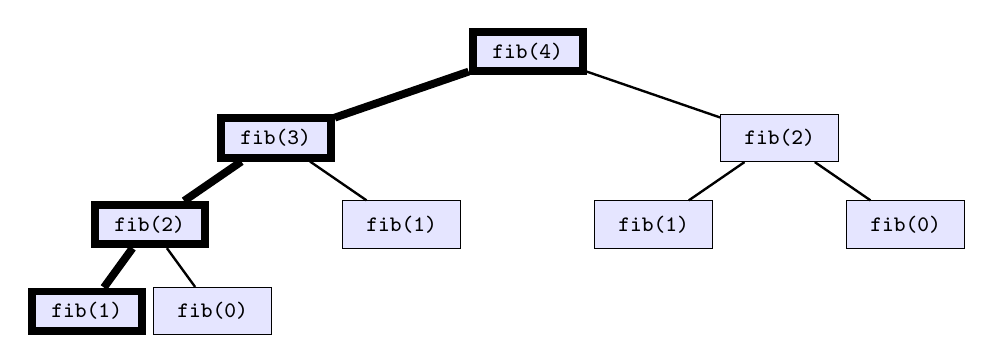
\begin{tikzpicture}

\draw (6.3500000000000005, 0.3)
  node[fill=blue!10,rounded corners=0cm,inner sep=0cm] {

\begin{minipage}[t][0.5cm]{1.4cm}
\mbox{}

\end{minipage}

};
\draw (6.3500000000000005, 0.3)
  node[draw, line width=0.1cm, , color=black,
       rounded corners=0cm, inner sep=0cm,
       name=A] {

\begin{minipage}[t][0.5cm]{1.4cm}
\mbox{}

\end{minipage}

};\draw (6.3500000000000005, 0.3) node[color=black] {\texttt{{\footnotesize \texttt{fib(4)}}}};
\draw (3.1500000000000004, -0.8)
  node[fill=blue!10,rounded corners=0cm,inner sep=0cm] {

\begin{minipage}[t][0.5cm]{1.4cm}
\mbox{}

\end{minipage}

};
\draw (3.1500000000000004, -0.8)
  node[draw, line width=0.1cm, , color=black,
       rounded corners=0cm, inner sep=0cm,
       name=B] {

\begin{minipage}[t][0.5cm]{1.4cm}
\mbox{}

\end{minipage}

};\draw (3.1500000000000004, -0.8) node[color=black] {\texttt{{\footnotesize \texttt{fib(3)}}}};
\draw (9.55, -0.8)
  node[fill=blue!10,rounded corners=0cm,inner sep=0cm] {

\begin{minipage}[t][0.6cm]{1.5cm}
\mbox{}

\end{minipage}

};
\draw (9.55, -0.8)
  node[draw, , , color=black,
       rounded corners=0cm, inner sep=0cm,
       name=I] {

\begin{minipage}[t][0.6cm]{1.5cm}
\mbox{}

\end{minipage}

};\draw (9.55, -0.8) node[color=black] {\texttt{{\footnotesize \texttt{fib(2)}}}};
\draw (1.5499999999999998, -1.9000000000000001)
  node[fill=blue!10,rounded corners=0cm,inner sep=0cm] {

\begin{minipage}[t][0.5cm]{1.4cm}
\mbox{}

\end{minipage}

};
\draw (1.5499999999999998, -1.9000000000000001)
  node[draw, line width=0.1cm, , color=black,
       rounded corners=0cm, inner sep=0cm,
       name=C] {

\begin{minipage}[t][0.5cm]{1.4cm}
\mbox{}

\end{minipage}

};\draw (1.5499999999999998, -1.9000000000000001) node[color=black] {\texttt{{\footnotesize \texttt{fib(2)}}}};
\draw (4.75, -1.9000000000000001)
  node[fill=blue!10,rounded corners=0cm,inner sep=0cm] {

\begin{minipage}[t][0.6cm]{1.5cm}
\mbox{}

\end{minipage}

};
\draw (4.75, -1.9000000000000001)
  node[draw, , , color=black,
       rounded corners=0cm, inner sep=0cm,
       name=F] {

\begin{minipage}[t][0.6cm]{1.5cm}
\mbox{}

\end{minipage}

};\draw (4.75, -1.9000000000000001) node[color=black] {\texttt{{\footnotesize \texttt{fib(1)}}}};
\draw (7.949999999999999, -1.9000000000000001)
  node[fill=blue!10,rounded corners=0cm,inner sep=0cm] {

\begin{minipage}[t][0.6cm]{1.5cm}
\mbox{}

\end{minipage}

};
\draw (7.949999999999999, -1.9000000000000001)
  node[draw, , , color=black,
       rounded corners=0cm, inner sep=0cm,
       name=G] {

\begin{minipage}[t][0.6cm]{1.5cm}
\mbox{}

\end{minipage}

};\draw (7.949999999999999, -1.9000000000000001) node[color=black] {\texttt{{\footnotesize \texttt{fib(1)}}}};
\draw (11.15, -1.9000000000000001)
  node[fill=blue!10,rounded corners=0cm,inner sep=0cm] {

\begin{minipage}[t][0.6cm]{1.5cm}
\mbox{}

\end{minipage}

};
\draw (11.15, -1.9000000000000001)
  node[draw, , , color=black,
       rounded corners=0cm, inner sep=0cm,
       name=H] {

\begin{minipage}[t][0.6cm]{1.5cm}
\mbox{}

\end{minipage}

};\draw (11.15, -1.9000000000000001) node[color=black] {\texttt{{\footnotesize \texttt{fib(0)}}}};
\draw (0.75, -3.0)
  node[fill=blue!10,rounded corners=0cm,inner sep=0cm] {

\begin{minipage}[t][0.5cm]{1.4cm}
\mbox{}

\end{minipage}

};
\draw (0.75, -3.0)
  node[draw, line width=0.1cm, , color=black,
       rounded corners=0cm, inner sep=0cm,
       name=D] {

\begin{minipage}[t][0.5cm]{1.4cm}
\mbox{}

\end{minipage}

};\draw (0.75, -3.0) node[color=black] {\texttt{{\footnotesize \texttt{fib(1)}}}};
\draw (2.35, -3.0)
  node[fill=blue!10,rounded corners=0cm,inner sep=0cm] {

\begin{minipage}[t][0.6cm]{1.5cm}
\mbox{}

\end{minipage}

};
\draw (2.35, -3.0)
  node[draw, , , color=black,
       rounded corners=0cm, inner sep=0cm,
       name=E] {

\begin{minipage}[t][0.6cm]{1.5cm}
\mbox{}

\end{minipage}

};\draw (2.35, -3.0) node[color=black] {\texttt{{\footnotesize \texttt{fib(0)}}}};\draw[line width=0.1cm,black] (A) to  (B);
\draw[line width=0.03cm,black] (A) to  (I);
\draw[line width=0.1cm,black] (B) to  (C);
\draw[line width=0.03cm,black] (B) to  (F);
\draw[line width=0.1cm,black] (C) to  (D);
\draw[line width=0.03cm,black] (C) to  (E);
\draw[line width=0.03cm,black] (I) to  (G);
\draw[line width=0.03cm,black] (I) to  (H);
\end{tikzpicture}

\end{center}


i.e., it's $4A$.
In general, the space complexity of \verb!f(n)! is
\[
\mathsc{Space}(n) = O(n)
\]

%-*-latex-*-

\begin{ex} 
  \label{ex:prob-00}
  \tinysidebar{\debug{exercises/{disc-prob-28/question.tex}}}

  \solutionlink{sol:prob-00}
  \qed
\end{ex} 
\begin{python0}
from solutions import *
add(label="ex:prob-00",
    srcfilename='exercises/discrete-probability/prob-00/answer.tex') 
\end{python0}


